%! Author = Philipp Emmenegger
%! Date = 30/06/2021

\section{Virtualization}
Creation of a virtual machine that acts like a real computer with an operating system.\\
\textbf{Host:} machine where the virtualization SW runs.\\
\textbf{Guest:} VM\\
\textbf{Hypervisor:} runs VM
\begin{itemize}
    \item Type 1: bare-metal e.g. Xen
    \item Type 2: hosted e.g. VirtualBox
\end{itemize}
\textbf{Needs to be the same architecture}
\begin{itemize}
    \item Otherwise emulation needed
\end{itemize}
\textbf{Virtual desktop infrastructure (VDI)}
\begin{itemize}
    \item Interact with a VM over a network
\end{itemize}
\textbf{Containers}
\begin{itemize}
    \item Isolated user-space instances
    \item Share the OS
\end{itemize}

\subsection{VM vs. Container}
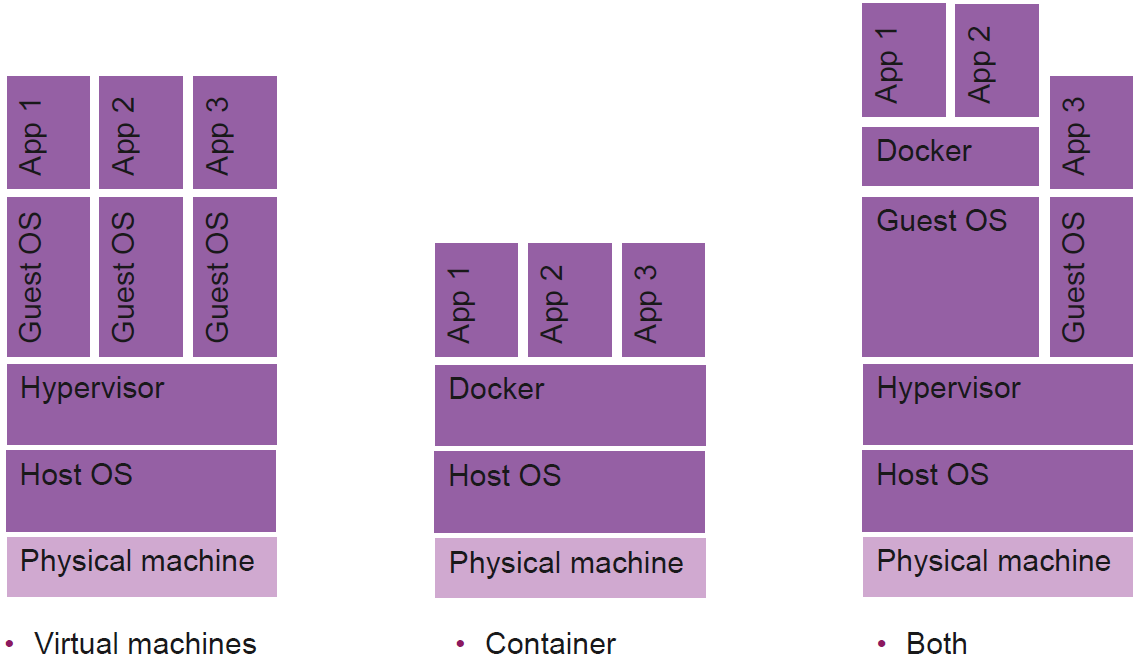
\includegraphics[width=\linewidth]{img/vm_container.png}
\begin{itemize}
    \item Containers are more agile than VMs
    \item Containers enable hybrid and multi-cloud adoption
    \item Integrate Containers with your existing IT processes
    \item Containers safe on VM licensing
\end{itemize}

\subsubsection{Container}
+ Reduced IT management resources\\
+ Reduced size of snapshots\\
+ Quicker spinning up apps\\
+/- Available memory is shared\\
+/- Process-based isolation (share same kernel)\\
\textbf{Use case:} complex application setup, with container less complex config

\subsubsection{Virtual Machine}
+ App can access all OS resources\\
+ Live migrations\\
+/- Pre allocates memory\\
+/- Full isolation\\
\textbf{Use case:} better hardware utilization / resource sharing

\subsection{Docker}
\begin{itemize}
    \item Containerization platform
    \item Software delivery framework
    \item Packages software into containers
    \item Provides OS-level virtualization
    \item Containers are isolated from each other
\end{itemize}
\textbf{Docker Compose}
\begin{itemize}
    \item Deploy multiple containers
\end{itemize}